\documentclass[12pt,a4paper,oneside]{report}
\newif\ifchronologia
\ifdefined\Chronologia\chronologiatrue\else\chronologiafalse\fi

% Typografia wzorowana na „Miara i całka” G. Plebanka:
% PL Roman, 12 pt, A4, klasyczne rozdziały i podrozdziały.
\usepackage[utf8]{inputenc}
\usepackage[OT4,plmath]{polski}
\usepackage{amsmath,amssymb,amsthm}
\usepackage[left=30.56mm,right=26.2mm,top=30mm,bottom=28mm]{geometry}
\usepackage{microtype}
\usepackage{graphicx}
\usepackage{eso-pic}
\usepackage{float}
\usepackage{enumitem}
\usepackage[hidelinks,unicode]{hyperref}

\hypersetup{
  pdftitle={Rachunek prawdopodobieństwa},
  pdfsubject={Skrypt z wykładów},
  linktoc=all,
  bookmarksnumbered=true
}
\graphicspath{{../grafika/}}
\setcounter{tocdepth}{1}
\setcounter{secnumdepth}{2}
\setlength{\parindent}{1.5em}
\setlength{\parskip}{0pt}
\setlist[enumerate]{label=\arabic*),leftmargin=2.1em,itemsep=0.25em}
\allowdisplaybreaks[1]

\theoremstyle{definition}
% Każdy rodzaj ma osobny licznik, ciągły przez cały rozdział.
\newtheorem{definicja}{Definicja}[chapter]
\newtheorem{przyklad}{Przykład}[chapter]
\newtheorem{uwaga}{Uwaga}[chapter]
\theoremstyle{plain}
\newtheorem{fakt}{Fakt}[chapter]
\newtheorem{twierdzenie}{Twierdzenie}[chapter]
\newtheorem{lemat}{Lemat}[chapter]
\newtheorem{wniosek}{Wniosek}[chapter]
\renewcommand{\proofname}{Dowód}

% Znaczniki nie zmieniają rozdziałów, sekcji ani liczników matematycznych.
\newcommand{\poczatekwykladu}[1]{%
  \ifchronologia
    \par\addvspace{\baselineskip}%
    \phantomsection
    \addcontentsline{toc}{section}{Wykład #1}%
    \noindent{\large\bfseries Wykład #1}\par\nobreak
    \noindent\rule{\linewidth}{0.4pt}\par\nobreak
    \addvspace{0.5\baselineskip}%
  \fi
}


\newcommand{\R}{\mathbb{R}}
\newcommand{\Q}{\mathbb{Q}}
\newcommand{\PP}{\mathbb{P}}
\newcommand{\F}{\mathcal{F}}
\newcommand{\B}{\mathcal{B}}
\DeclareMathOperator{\pole}{pole}


\begin{document}

\hypersetup{pageanchor=false}
% Wspólna okładka; na drugiej stronie informacja właściwa dla wariantu.
\begin{titlepage}
  \thispagestyle{empty}
  \AddToShipoutPictureBG*{%
    \AtPageLowerLeft{%
      % Import natywny pdfTeX zachowuje pojedynczą grupę przezroczystości.
      % Sterownik graphicx dodawał drugą /Group do tej przezroczystej strony.
      \pdfximage width\paperwidth height\paperheight {../grafika/okladka.pdf}%
      \pdfrefximage\pdflastximage
    }%
  }
  \null
\end{titlepage}

\begin{titlepage}
  \thispagestyle{empty}
  \centering
  \vspace*{\fill}
  \begin{minipage}{\textwidth}
    \centering
    \fontsize{17}{25}\selectfont
    Skrypt do wykładu prof. Jacka Małeckiego\\
    \ifchronologia
      z oznaczeniem chronologii wykładu,\\
    \else
      bez oznaczenia chronologii wykładu,\\
    \fi
    wykonane przez Szymona Gazińskiego
  \end{minipage}
  \vspace*{\fill}
\end{titlepage}


\pagenumbering{roman}
\hypersetup{pageanchor=true}
\pdfbookmark[0]{Spis treści}{spis-tresci}
\tableofcontents
\clearpage
\pagenumbering{arabic}
\pagestyle{plain}

% Źródła: materialy/2026-10-05/notatki.pdf oraz tablica-01, -02, -03.jpeg.
\chapter{Aksjomatyczna definicja prawdopodobieństwa}
\label{chap:aksjomaty}

\section{Przestrzeń probabilistyczna}
\label{sec:przestrzen}

\begin{definicja}
\emph{Przestrzenią probabilistyczną} nazywamy trójkę
$(\Omega,\F,\PP)$, gdzie:
\begin{enumerate}
  \item $\Omega$ jest niepustym zbiorem, zwanym \emph{przestrzenią
    stanów elementarnych};
  \item $\F$ jest rodziną podzbiorów $\Omega$ taką, że:
    \begin{align*}
      &\varnothing\in\F,\\
      &A\in\F\ \Longrightarrow\ A^c\in\F,\\
      &A_1,A_2,\ldots\in\F\ \Longrightarrow\
        \bigcup_{n=1}^{\infty}A_n\in\F;
    \end{align*}
  \item $\PP\colon\F\to[0,1]$ jest funkcją spełniającą warunki:
    \begin{align}
      \PP(\Omega)&=1,\label{eq:normalizacja}\\
      \PP\!\left(\bigcup_{n=1}^{\infty}A_n\right)
        &=\sum_{n=1}^{\infty}\PP(A_n),
        \label{eq:addytywnosc}
    \end{align}
    przy czym wzór \eqref{eq:addytywnosc} obowiązuje dla każdej
    rodziny $A_1,A_2,\ldots\in\F$ zdarzeń parami rozłącznych, czyli
    $A_i\cap A_j=\varnothing$ dla $i\ne j$.
\end{enumerate}
Rodzinę $\F$ nazywamy \emph{$\sigma$-ciałem}, a jej elementy
\emph{zdarzeniami}. Funkcję $\PP$ nazywamy \emph{prawdopodobieństwem}.
Warunek \eqref{eq:addytywnosc} to \emph{przeliczalna addytywność}.
\end{definicja}

\begin{uwaga}
Przyjmujemy następującą terminologię:
\begin{enumerate}
  \item $\omega\in\Omega$ jest stanem elementarnym.
  \item Zdarzenia $A,B\in\F$ \emph{wykluczają się}, jeżeli
    $A\cap B=\varnothing$.
  \item $A^c=\Omega\setminus A$ jest \emph{zdarzeniem przeciwnym}
    do zdarzenia $A$.
  \item $\varnothing$ jest \emph{zdarzeniem niemożliwym},
    a $\Omega$ jest \emph{zdarzeniem pewnym}.
\end{enumerate}
\end{uwaga}

\begin{fakt}
\label{fakt:pusty}
Prawdopodobieństwo zdarzenia niemożliwego wynosi zero:
\[
  \PP(\varnothing)=0.
\]
\end{fakt}

\section{Zbiory borelowskie i miara Lebesgue'a}
\label{sec:borel}

\begin{definicja}
\emph{$\sigma$-ciałem zbiorów borelowskich} na $\R$
(odpowiednio na $\R^2$ lub $\R^n$) nazywamy najmniejsze
$\sigma$-ciało zawierające wszystkie zbiory otwarte.
Oznaczamy je przez $\B(\R)$ (odpowiednio $\B(\R^2)$ lub $\B(\R^n)$).
Na prostej wystarczy rozważać otwarte przedziały $(a,b)$.
Elementy tego $\sigma$-ciała nazywamy \emph{zbiorami borelowskimi}.
\end{definicja}

Na przestrzeni $(\R,\B(\R))$ istnieje miara $\lambda$ taka, że
\[
  \lambda\bigl((a,b)\bigr)=b-a
  \qquad\text{dla }a<b.
\]
Jest to \emph{miara Lebesgue'a}. Mierzy ona długość i spełnia
warunek przeliczalnej addytywności:
\[
  \lambda\!\left(\bigcup_{n=1}^{\infty}A_n\right)
    =\sum_{n=1}^{\infty}\lambda(A_n)
\]
dla zbiorów borelowskich $A_n$ parami rozłącznych.

\begin{fakt}
\label{fakt:miara-zero}
Każdy zbiór jednopunktowy ma miarę Lebesgue'a równą zero:
\[
  \lambda(\{x\})=0\qquad\text{dla każdego }x\in\R.
\]
W szczególności $\lambda(\Q)=0$.
\end{fakt}

Istotnie, zbiór liczb wymiernych jest przeliczalny. Jeśli
$\Q=\{q_1,q_2,\ldots\}$, przy czym liczby $q_i$ są różne, to
\[
  \lambda(\Q)
    =\lambda\!\left(\bigcup_{i=1}^{\infty}\{q_i\}\right)
    =\sum_{i=1}^{\infty}\lambda(\{q_i\})
    =0.
\]

\section{Prawdopodobieństwo geometryczne}
\label{sec:geometryczne}

Niech $\Omega\subseteq\R$ będzie zbiorem borelowskim, dla którego
$0<\lambda(\Omega)<\infty$. Przyjmujemy
\[
  \F=\{A\cap\Omega:A\in\B(\R)\}.
\]
Dla każdego $B\in\F$ definiujemy
\begin{equation}
  \PP(B)=\frac{\lambda(B)}{\lambda(\Omega)}.
  \label{eq:geometryczne}
\end{equation}
W ten sposób otrzymujemy przestrzeń probabilistyczną
$(\Omega,\F,\PP)$.

Analogicznie, dla borelowskiego zbioru $\Omega\subseteq\R^2$
o dodatnim i skończonym polu, prawdopodobieństwo zdarzenia
$A\in\{B\cap\Omega:B\in\B(\R^2)\}$ określamy wzorem
\begin{equation}
  \PP(A)=\frac{\pole(A)}{\pole(\Omega)}.
  \label{eq:pole}
\end{equation}

\section{Przykład: suma dwóch losowanych liczb}
\label{sec:suma}

\begin{przyklad}
Losujemy niezależnie i jednostajnie dwie liczby z przedziału $[0,1]$.
Jakie jest prawdopodobieństwo, że ich suma jest większa od $1/2$?
\end{przyklad}

\noindent\emph{Rozwiązanie.}
Przestrzenią stanów elementarnych jest kwadrat jednostkowy
\[
  \Omega=[0,1]^2=\{(x,y):x,y\in[0,1]\}.
\]
Rozważamy zdarzenie
\[
  A=\{(x,y)\in[0,1]^2:x+y>\tfrac12\}.
\]
Jego dopełnienie $A^c$ jest trójkątem o wierzchołkach
$(0,0)$, $(1/2,0)$ i $(0,1/2)$, przedstawionym na
rysunku~\ref{fig:suma}. Stąd
\[
  \pole(A^c)=\frac12\cdot\frac12\cdot\frac12=\frac18,
  \qquad \pole(\Omega)=1.
\]
Korzystając ze wzoru \eqref{eq:pole}, otrzymujemy
\begin{equation}
  \PP(A)=1-\PP(A^c)
    =1-\frac{\pole(A^c)}{\pole(\Omega)}
    =1-\frac18=\boxed{\frac78}.
  \label{eq:wynik-suma}
\end{equation}

\begin{figure}[htbp]
  \centering
  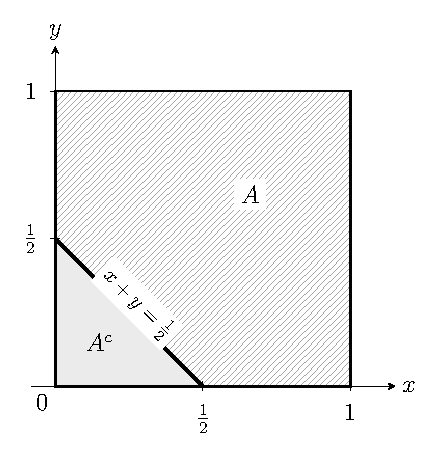
\includegraphics[width=7.6cm]{suma-dwoch-liczb.pdf}
  \caption{Kwadrat $\Omega=[0,1]^2$ oraz zdarzenia
    $A=\{x+y>1/2\}$ i $A^c=\{x+y\leq1/2\}$.}
  \label{fig:suma}
\end{figure}

\begin{uwaga}
Na tablicy zapisano $x+y\geq1/2$. Odcinek $x+y=1/2$ ma pole
równe zero, więc zastąpienie znaku $>$ znakiem $\geq$
nie zmienia wyniku.
\end{uwaga}

% Źródła: materialy/2026-10-12/wlasnosci-zeszyt.png i IMG_6916.jpeg.
% Numeracja 6, 7 według tablicy; podaddytywność w punkcie 5.
\section{Własności prawdopodobieństwa}
\label{sec:wlasnosci}

\begin{twierdzenie}
\label{tw:wlasnosci}
Niech $(\Omega,\F,\PP)$ będzie przestrzenią probabilistyczną.
Wówczas zachodzą następujące własności.
\begin{enumerate}[label=\arabic*),ref=\arabic*]
  \item\label{wlasn:zakres}
    Dla każdego $A\in\F$ zachodzi
    \[
      0\leq\PP(A)\leq1.
    \]
  \item\label{wlasn:pewne}
    Zdarzenie niemożliwe i zdarzenie pewne mają prawdopodobieństwa
    \[
      \PP(\varnothing)=0,\qquad \PP(\Omega)=1.
    \]
  \item\label{wlasn:dopelnienie}
    Dla każdego $A\in\F$ zachodzi
    \[
      \PP(A^c)=1-\PP(A).
    \]
  \item\label{wlasn:monotonicznosc}
    Jeżeli $A,B\in\F$ oraz $A\subseteq B$, to
    \[
      \PP(A)\leq\PP(B).
    \]
  \item\label{wlasn:suma}
    Dla $A,B\in\F$ mamy
    \[
      \PP(A\cup B)=\PP(A)+\PP(B)-\PP(A\cap B)
        \leq\PP(A)+\PP(B).
    \]
    Ogólniej, dla dowolnych zdarzeń $A_1,A_2,\ldots\in\F$
    zachodzi \emph{przeliczalna podaddytywność}:
    \[
      \PP\!\left(\bigcup_{n=1}^{\infty}A_n\right)
        \leq\sum_{n=1}^{\infty}\PP(A_n).
    \]
  \item\label{wlasn:rosnacy}
    Jeżeli $A_1\subseteq A_2\subseteq\cdots$ jest rosnącym
    ciągiem zdarzeń, to
    \begin{equation}
      \PP\!\left(\bigcup_{n=1}^{\infty}A_n\right)
        =\lim_{n\to\infty}\PP(A_n).
      \label{eq:ciag-rosnacy}
    \end{equation}
  \item\label{wlasn:malejacy}
    Jeżeli $A_1\supseteq A_2\supseteq\cdots$ jest malejącym
    ciągiem zdarzeń, to
    \begin{equation}
      \PP\!\left(\bigcap_{n=1}^{\infty}A_n\right)
        =\lim_{n\to\infty}\PP(A_n).
      \label{eq:ciag-malejacy}
    \end{equation}
\end{enumerate}
\end{twierdzenie}

% Wszystkie stwierdzenia powyżej należą do wykładu 1.
% Według polecenia użytkownika wykład 2 zaczyna się od dowodu 6.
\poczatekwykladu{2}

\begin{proof}[Dowód własności \ref{wlasn:rosnacy}]
Przyjmijmy $A_0=\varnothing$ i zdefiniujmy
\[
  B_n=A_n\setminus A_{n-1},\qquad n=1,2,\ldots.
\]
Zdarzenia $B_n$ są parami rozłączne; ilustruje to
rysunek~\ref{fig:ciag-rosnacy}. Ponadto dla każdego $N\geq1$
\[
  \bigcup_{n=1}^{N}B_n=\bigcup_{n=1}^{N}A_n=A_N,
  \qquad
  \bigcup_{n=1}^{\infty}B_n=\bigcup_{n=1}^{\infty}A_n.
\]
Z przeliczalnej addytywności otrzymujemy
\begin{align*}
  \PP\!\left(\bigcup_{n=1}^{\infty}A_n\right)
    &=\PP\!\left(\bigcup_{n=1}^{\infty}B_n\right)
      =\sum_{n=1}^{\infty}\PP(B_n)\\
    &=\lim_{N\to\infty}\sum_{n=1}^{N}\PP(B_n)
      =\lim_{N\to\infty}\PP\!\left(\bigcup_{n=1}^{N}B_n\right)\\
    &=\lim_{N\to\infty}\PP(A_N).
\end{align*}
\end{proof}

\begin{figure}[H]
  \centering
  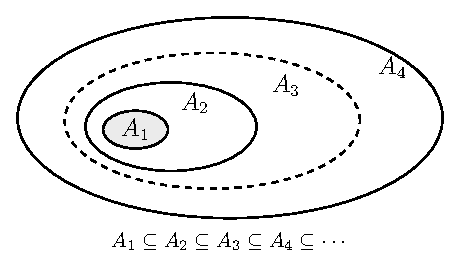
\includegraphics[width=8.2cm]{ciag-zdarzen-rosnacy.pdf}
  \caption{Rosnący ciąg zdarzeń. Kolejne różnice
    $B_n=A_n\setminus A_{n-1}$ są parami rozłączne.}
  \label{fig:ciag-rosnacy}
\end{figure}

\begin{proof}[Dowód własności \ref{wlasn:malejacy}]
Skoro $A_1\supseteq A_2\supseteq\cdots$, to
$A_1^c\subseteq A_2^c\subseteq\cdots$. Korzystamy z prawa
de Morgana oraz z udowodnionej własności \ref{wlasn:rosnacy}:
\begin{align*}
  \PP\!\left(\bigcap_{n=1}^{\infty}A_n\right)
    &=1-\PP\!\left(\left(\bigcap_{n=1}^{\infty}A_n\right)^c\right)\\
    &=1-\PP\!\left(\bigcup_{n=1}^{\infty}A_n^c\right)\\
    &=1-\lim_{n\to\infty}\PP(A_n^c)
      =\lim_{n\to\infty}\bigl(1-\PP(A_n^c)\bigr)\\
    &=\lim_{n\to\infty}\PP(A_n).
\end{align*}
\end{proof}

% Źródła: materialy/2026-10-12/notatki.pdf i zdjęcia IMG_6917--IMG_6922.
\chapter{Prawdopodobieństwo warunkowe}
\label{chap:warunkowe}

\section{Definicja i podstawowe własności}
\label{sec:warunkowe}

Niech $(\Omega,\F,\PP)$ będzie przestrzenią probabilistyczną.

\begin{definicja}
\label{def:warunkowe}
Dla zdarzeń $A,B\in\F$ takich, że $\PP(B)>0$,
\emph{prawdopodobieństwo warunkowe zdarzenia $A$ pod warunkiem $B$}
definiujemy wzorem
\begin{equation}
  \PP(A\mid B)=\frac{\PP(A\cap B)}{\PP(B)}.
  \label{eq:warunkowe}
\end{equation}
\end{definicja}

\begin{uwaga}
Przy ustalonym $B\in\F$ o dodatnim prawdopodobieństwie wzór
\[
  \PP_B(A)=\PP(A\mid B),\qquad A\in\F,
\]
definiuje nowe prawdopodobieństwo na $(\Omega,\F)$.
\end{uwaga}

\begin{fakt}
\label{fakt:wlasnosci-warunkowego}
Niech $A,B\in\F$ oraz $\PP(B)>0$. Wówczas:
\begin{enumerate}
  \item jeśli $A\subseteq B$, to
    \[
      \PP(A\mid B)=\frac{\PP(A)}{\PP(B)};
    \]
  \item jeśli $B\subseteq A$, to $\PP(A\mid B)=1$;
  \item jeśli $A\cap B=\varnothing$, to $\PP(A\mid B)=0$;
    ogólniej, wystarczy warunek $\PP(A\cap B)=0$;
  \item jeśli $C\in\F$ i $\PP(B\cap C)>0$, to
    \begin{equation}
      \PP(A\mid B\cap C)
        =\frac{\PP(A\cap B\mid C)}{\PP(B\mid C)}.
      \label{eq:warunkowanie-dwukrotne}
    \end{equation}
\end{enumerate}
\end{fakt}

\begin{przyklad}[Rodzina z dwojgiem dzieci]
\label{przykl:dzieci}
Wybieramy rodzinę z dwojgiem dzieci. Jakie jest prawdopodobieństwo,
że ma ona dwóch chłopców, jeśli:
\begin{enumerate}[label=\alph*)]
  \item starsze dziecko jest chłopcem;
  \item w rodzinie jest co najmniej jeden chłopiec?
\end{enumerate}
Zakładamy, że płcie dzieci są niezależne, a każda z dwóch płci ma
prawdopodobieństwo $1/2$.
\end{przyklad}

\noindent\emph{Rozwiązanie.}
Kodujemy chłopca przez $0$, a dziewczynkę przez $1$. Pierwsza współrzędna
odpowiada starszemu dziecku. Cztery stany elementarne
\[
  \Omega=\{(0,0),(0,1),(1,0),(1,1)\}
\]
są jednakowo prawdopodobne. Przyjmujemy
\begin{align*}
  A&=\{(0,0)\},\\
  B_1&=\{(0,0),(0,1)\},\\
  B_2&=\{(0,0),(0,1),(1,0)\}.
\end{align*}
Ponieważ $A\subseteq B_1$ i $A\subseteq B_2$, otrzymujemy
\[
  \PP(A\mid B_1)=\frac{1/4}{1/2}=\frac12,
  \qquad
  \PP(A\mid B_2)=\frac{1/4}{3/4}=\frac13.
\]

\section{Prawdopodobieństwo całkowite}
\label{sec:calkowite}

\begin{definicja}
\label{def:rozbicie}
\emph{Rozbiciem przestrzeni $\Omega$} nazywamy rodzinę zbiorów
$(B_n)_{n\in I}$, gdzie $I\subseteq\mathbb{N}$ jest zbiorem indeksów,
taką, że:
\begin{enumerate}
  \item $B_n\cap B_m=\varnothing$ dla $n,m\in I$, $n\ne m$;
  \item $\displaystyle\bigcup_{n\in I}B_n=\Omega$.
\end{enumerate}
Rozbicie może być skończone lub przeliczalne.
\end{definicja}

\begin{twierdzenie}[O prawdopodobieństwie całkowitym]
\label{tw:calkowite}
Niech $(B_n)_{n\in I}$ będzie rozbiciem $\Omega$ takim, że
$B_n\in\F$ i $\PP(B_n)>0$ dla każdego $n\in I$.
Wówczas dla dowolnego $A\in\F$ zachodzi
\begin{equation}
  \PP(A)=\sum_{n\in I}\PP(A\mid B_n)\PP(B_n).
  \label{eq:calkowite}
\end{equation}
\end{twierdzenie}

\begin{proof}
Zdarzenia $A\cap B_n$ są parami rozłączne. Zatem
\begin{align*}
  \PP(A)
    &=\PP(A\cap\Omega)
      =\PP\!\left(A\cap\bigcup_{n\in I}B_n\right)\\
    &=\PP\!\left(\bigcup_{n\in I}(A\cap B_n)\right)
      =\sum_{n\in I}\PP(A\cap B_n)\\
    &=\sum_{n\in I}\PP(A\mid B_n)\PP(B_n).
\end{align*}
\end{proof}

\begin{przyklad}[Zniszczenie celu]
\label{przykl:strzaly}
Prawdopodobieństwo trafienia w cel wynosi $1/2$, a wyniki kolejnych
strzałów są niezależne. Prawdopodobieństwo zniszczenia celu przy
dokładnie $k$ celnych strzałach wynosi $1-(1/3)^k$.
Jakie jest prawdopodobieństwo zniszczenia celu po oddaniu dziesięciu strzałów?
\end{przyklad}

\noindent\emph{Rozwiązanie.}
Niech $A$ oznacza zniszczenie celu, a $B_i$ zdarzenie, że dokładnie
$i$ spośród dziesięciu strzałów jest celnych, gdzie $i=0,1,\ldots,10$.
Wówczas
\[
  \PP(A\mid B_i)=1-\left(\frac13\right)^i,
  \qquad
  \PP(B_i)=\binom{10}{i}\left(\frac12\right)^{10}.
\]
Korzystając ze wzoru \eqref{eq:calkowite} i ze wzoru dwumianowego
\[
  (a+b)^n=\sum_{i=0}^{n}\binom{n}{i}a^ib^{n-i},
\]
otrzymujemy
\begin{align*}
  \PP(A)
    &=\sum_{i=0}^{10}\left(1-\left(\frac13\right)^i\right)
        \binom{10}{i}\left(\frac12\right)^{10}\\
    &=\sum_{i=0}^{10}\binom{10}{i}\left(\frac12\right)^{10}
      -\sum_{i=0}^{10}\binom{10}{i}
        \left(\frac16\right)^i\left(\frac12\right)^{10-i}\\
    &=1-\left(\frac16+\frac12\right)^{10}
      =\boxed{1-\left(\frac23\right)^{10}}.
\end{align*}

\begin{przyklad}[Dwie urny]
\label{przykl:urny}
Mamy dwie urny, każda zawiera sto kul. Jedna kula jest biała:
trafia do pierwszej urny z prawdopodobieństwem $2/3$, a do drugiej
z prawdopodobieństwem $1/3$. Pozostałe kule są czarne.
Wykonujemy osiemdziesiąt losowań ze zwracaniem.
Jak rozdzielić losowania między urny, aby zmaksymalizować
prawdopodobieństwo wylosowania białej kuli co najmniej raz?
\end{przyklad}

\noindent\emph{Rozwiązanie.}
Niech $B_i$ oznacza zdarzenie, że biała kula znajduje się w $i$-tej urnie,
a $A$ zdarzenie, że zostanie wylosowana co najmniej raz.
Wykonujemy $k$ losowań z pierwszej urny i $m=80-k$ z drugiej.
Oznaczmy przez $q=99/100$ prawdopodobieństwo wylosowania czarnej kuli
z urny zawierającej białą kulę. Wówczas
\[
  \PP(A\mid B_1)=1-q^k,
  \qquad
  \PP(A\mid B_2)=1-q^{80-k}.
\]
Ze wzoru \eqref{eq:calkowite} otrzymujemy
\begin{equation}
  \PP(A)=f(k)=\frac23(1-q^k)+\frac13(1-q^{80-k}),
  \qquad k\in\{0,1,\ldots,80\}.
  \label{eq:urny-funkcja}
\end{equation}
Aby znaleźć maksimum, rozważamy najpierw zmienną rzeczywistą $x\in[0,80]$.
Liczymy
\[
  f'(x)=\frac{\ln q}{3}\bigl(q^{80-x}-2q^x\bigr).
\]
Warunek $f'(x)=0$ jest równoważny
\[
  q^{80-2x}=2,
  \qquad
  x=\frac12\left(80-\frac{\ln2}{\ln q}\right)\approx74{,}484.
\]
Ponieważ
\[
  f''(x)=-\frac{(\ln q)^2}{3}\bigl(q^{80-x}+2q^x\bigr)<0,
\]
jest to jedyny punkt maksimum. Dla całkowitej liczby losowań
porównujemy dwóch kandydatów:
\[
  f(74)\approx0{,}3692799222,
  \qquad f(75)\approx0{,}3692788890.
\]
Najlepiej wykonać \emph{74 losowania z pierwszej urny i 6 z drugiej}.
Oba powyższe prawdopodobieństwa po zaokrągleniu do czterech miejsc
po przecinku wynoszą $0{,}3693$.

\section{Wzór Bayesa}
\label{sec:bayes}

\begin{twierdzenie}[Wzór Bayesa]
\label{tw:bayes}
Niech $(B_n)_{n\in I}$ będzie rozbiciem $\Omega$ takim, że
$B_n\in\F$ i $\PP(B_n)>0$ dla każdego $n\in I$.
Jeżeli $A\in\F$ i $\PP(A)>0$, to dla każdego $n\in I$
\begin{equation}
  \PP(B_n\mid A)
    =\frac{\PP(A\mid B_n)\PP(B_n)}{\PP(A)}
    =\frac{\PP(A\mid B_n)\PP(B_n)}
      {\displaystyle\sum_{k\in I}\PP(A\mid B_k)\PP(B_k)}.
  \label{eq:bayes}
\end{equation}
\end{twierdzenie}

\begin{przyklad}[ZONK]
\label{przykl:zonk}
Za jedną z trzech bramek znajduje się nagroda, a za pozostałymi dwoma
zonki. Każda bramka zawiera nagrodę z prawdopodobieństwem $1/3$.
Wybieramy pierwszą bramkę. Filip Chajzer zna położenie nagrody
i otwiera jedną z pozostałych bramek, zawsze pokazując zonka.
Jeżeli może otworzyć obie, wybiera każdą z prawdopodobieństwem $1/2$.
Chajzer otworzył trzecią bramkę. Jakie jest prawdopodobieństwo,
że nagroda znajduje się w drugiej bramce? Czy warto zmienić wybór?
\end{przyklad}

\noindent\emph{Rozwiązanie.}
Przyjmujemy oznaczenia
\[
  A=\{\text{Chajzer otwiera trzecią bramkę}\},
  \qquad
  B_i=\{\text{nagroda jest w $i$-tej bramce}\},
\]
gdzie $i=1,2,3$. Zdarzenia $B_1,B_2,B_3$ tworzą rozbicie $\Omega$,
a $\PP(B_i)=1/3$ dla każdego $i$.
Jeśli nagroda znajduje się w pierwszej bramce, prowadzący ma wybór
między drugą a trzecią. Jeśli znajduje się w drugiej, musi otworzyć
trzecią; jeśli w trzeciej, musi otworzyć drugą. Stąd
\[
  \PP(A\mid B_1)=\frac12,
  \qquad \PP(A\mid B_2)=1,
  \qquad \PP(A\mid B_3)=0.
\]
Ze wzoru na prawdopodobieństwo całkowite \eqref{eq:calkowite} mamy
\[
  \PP(A)=\frac12\cdot\frac13+1\cdot\frac13+0\cdot\frac13=\frac12.
\]
Zatem wzór Bayesa \eqref{eq:bayes} daje
\begin{equation}
  \PP(B_2\mid A)
    =\frac{\PP(A\mid B_2)\PP(B_2)}{\PP(A)}
    =\frac{1\cdot(1/3)}{1/2}=\boxed{\frac23}.
  \label{eq:zonk-wynik}
\end{equation}
Natomiast $\PP(B_1\mid A)=1/3$. Warto więc zmienić wybór z pierwszej
bramki na drugą: prawdopodobieństwo wygranej wzrasta z $1/3$ do $2/3$.

\begin{przyklad}[Moneta z dwoma orłami]
\label{przykl:moneta}
Mamy sto monet: dziewięćdziesiąt dziewięć uczciwych i jedną
z orłem na obu stronach. Wybieramy monetę losowo i rzucamy nią dziesięć razy.
Za każdym razem wypada orzeł. Jakie jest prawdopodobieństwo,
że wybraliśmy monetę z dwoma orłami?
\end{przyklad}

\noindent\emph{Rozwiązanie.}
Niech $A$ oznacza dziesięć orłów, $B_1$ wybór uczciwej monety,
a $B_2$ wybór monety z dwoma orłami. Wówczas
\begin{align*}
  \PP(B_1)&=\frac{99}{100},&
  \PP(B_2)&=\frac1{100},\\
  \PP(A\mid B_1)&=\left(\frac12\right)^{10},&
  \PP(A\mid B_2)&=1.
\end{align*}
Prawdopodobieństwo dziesięciu orłów wynosi
\[
  \PP(A)=\left(\frac12\right)^{10}\frac{99}{100}+\frac1{100}.
\]
Ze wzoru Bayesa \eqref{eq:bayes} otrzymujemy
\begin{equation}
  \PP(B_2\mid A)
    =\frac{1/100}{(1/2)^{10}\cdot99/100+1/100}
    =\frac{1024}{1123}\approx\boxed{0{,}9118}.
  \label{eq:moneta-wynik}
\end{equation}

% Źródła: materialy/2026-10-19/niezaleznosc.png i zdjęcia IMG_6950--IMG_6962.
\chapter{Niezależność}
\label{chap:niezaleznosc}

\poczatekwykladu{3}

\section{Niezależność dwóch zdarzeń}
\label{sec:niezaleznosc-dwoch}

Niech $(\Omega,\F,\PP)$ będzie przestrzenią probabilistyczną.

\begin{definicja}
\label{def:niezaleznosc-dwoch}
Zdarzenia $A,B\in\F$ są \emph{niezależne}, jeżeli
\begin{equation}
  \PP(A\cap B)=\PP(A)\PP(B).
  \label{eq:niezaleznosc-dwoch}
\end{equation}
\end{definicja}

\begin{uwaga}
Jeżeli $\PP(A)>0$ i zdarzenia $A,B$ są niezależne, to
\[
  \PP(B\mid A)=\frac{\PP(A\cap B)}{\PP(A)}
    =\frac{\PP(A)\PP(B)}{\PP(A)}=\PP(B).
\]
\end{uwaga}

\begin{przyklad}[Dwa rzuty kostką]
\label{przykl:kostka-niezaleznosc}
Rzucamy dwukrotnie uczciwą kostką; wyniki rzutów są niezależne.
Niech $A$ oznacza wyrzucenie szóstki w pierwszym rzucie,
$B$ wyrzucenie jedynki w drugim rzucie, a $C$ uzyskanie
parzystych wyników w obu rzutach. Sprawdźmy niezależność tych zdarzeń.
\end{przyklad}

\noindent\emph{Rozwiązanie.}
Przyjmujemy $\Omega=\{1,2,\ldots,6\}^2$ z jednakowo prawdopodobnymi
wynikami. Mamy
\[
  \PP(A)=\PP(B)=\frac16,
  \qquad \PP(C)=\frac12\cdot\frac12=\frac14.
\]
Ponadto
\begin{align*}
  \PP(A\cap B)&=\frac1{36}=\PP(A)\PP(B),\\
  \PP(A\cap C)&=\frac16\cdot\frac12=\frac1{12}
    \ne\frac1{24}=\PP(A)\PP(C),\\
  \PP(B\cap C)&=0\ne\frac1{24}=\PP(B)\PP(C).
\end{align*}
Zdarzenia $A$ i $B$ są niezależne, natomiast pary $A,C$ oraz $B,C$
nie są niezależne.

\begin{przyklad}[Rzuty monetą]
\label{przykl:moneta-niezaleznosc}
Rzucamy $n\geq2$ razy uczciwą monetą, niezależnie w kolejnych próbach.
Niech $A$ oznacza, że wypadła co najwyżej jedna reszka,
a $B$, że nie wypadły ani same orły, ani same reszki.
Dla jakich $n$ zdarzenia $A$ i $B$ są niezależne?
\end{przyklad}

\noindent\emph{Rozwiązanie.}
Wszystkie $2^n$ ciągów wyników są jednakowo prawdopodobne.
Zdarzenie $A$ obejmuje ciąg samych orłów oraz $n$ ciągów z jedną reszką,
więc
\[
  \PP(A)=\frac{1+n}{2^n},
  \qquad \PP(B)=1-\PP(B^c)=1-\frac2{2^n}.
\]
Dla $n\geq2$ zdarzenie $A\cap B$ oznacza dokładnie jedną reszkę,
stąd $\PP(A\cap B)=n/2^n$. Warunek niezależności jest równoważny
\begin{align*}
  \frac{n}{2^n}
    &=\frac{n+1}{2^n}\left(1-\frac2{2^n}\right),\\
  n2^n&=(n+1)(2^n-2),\\
  2(n+1)&=2^n,
  \qquad\text{czyli}\qquad n+1=2^{n-1}.
\end{align*}
Równość zachodzi dla $n=3$. Dla $n=2$ nie jest spełniona,
a dla $n\geq4$ mamy $2^{n-1}>n+1$ (nierówność utrzymuje się indukcyjnie).
Zatem \emph{zdarzenia są niezależne dokładnie dla $n=3$}.

\section{Niezależność rodzin zdarzeń}
\label{sec:niezaleznosc-rodzin}

\begin{definicja}
\label{def:niezaleznosc-rodziny}
Rodzina zdarzeń $(A_t)_{t\in T}$, gdzie $T$ jest dowolnym zbiorem indeksów,
jest \emph{niezależna}, jeżeli dla każdego $m\geq1$ i każdych parami różnych
$t_1,\ldots,t_m\in T$ zachodzi
\begin{equation}
  \PP\!\left(\bigcap_{i=1}^{m}A_{t_i}\right)
    =\prod_{i=1}^{m}\PP(A_{t_i}).
  \label{eq:niezaleznosc-rodziny}
\end{equation}
W szczególności zdarzenia $A_1,\ldots,A_n$ są niezależne, gdy
dla każdego $m\in\{2,\ldots,n\}$ i każdych indeksów
$1\leq t_1<\cdots<t_m\leq n$ spełniony jest wzór
\eqref{eq:niezaleznosc-rodziny}.
\end{definicja}

\begin{definicja}
\label{def:niezaleznosc-parami}
Zdarzenia $A_1,\ldots,A_n$ są \emph{parami niezależne}, jeżeli
\[
  \PP(A_i\cap A_j)=\PP(A_i)\PP(A_j)
  \qquad\text{dla wszystkich }i\ne j.
\]
\end{definicja}

\begin{definicja}
\label{def:dwie-rodziny}
Dwie rodziny zdarzeń $\mathcal{A},\mathcal{B}\subseteq\F$
są \emph{niezależne}, jeżeli dla każdych
$A\in\mathcal{A}$ oraz $B\in\mathcal{B}$ zachodzi
\[
  \PP(A\cap B)=\PP(A)\PP(B).
\]
\end{definicja}

\begin{definicja}
\label{def:rodzina-rodzin}
Rodziny zdarzeń $(\mathcal{A}_t)_{t\in T}$, gdzie
$\mathcal{A}_t\subseteq\F$, są \emph{niezależne}, jeżeli dla każdego
$m\geq1$, każdych parami różnych $t_1,\ldots,t_m\in T$ oraz dowolnych
zdarzeń $A_{t_i}\in\mathcal{A}_{t_i}$, $i=1,\ldots,m$, mamy
\[
  \PP(A_{t_1}\cap\cdots\cap A_{t_m})
    =\PP(A_{t_1})\cdots\PP(A_{t_m}).
\]
\end{definicja}

\begin{przyklad}[Niezależność parami nie wystarcza]
\label{przykl:niezaleznosc-parami}
Losujemy niezależnie i jednostajnie dwie liczby $x,y$ z odcinka $[0,1]$.
Przyjmujemy model geometryczny na $\Omega=[0,1]^2$ i zdarzenia
\begin{align*}
  A&=\{(x,y)\in\Omega:x\geq\tfrac12\},\\
  B&=\{(x,y)\in\Omega:y\geq\tfrac12\},\\
  C&=\{(x,y)\in\Omega:
    \min\{x,y\}>\tfrac12\ \text{lub}\ \max\{x,y\}\leq\tfrac12\}.
\end{align*}
Czy zdarzenia $A,B,C$ są niezależne?
\end{przyklad}

\noindent\emph{Rozwiązanie.}
Zdarzenie $C$ zajmuje dwa kwadraty leżące po przekątnej kwadratu
jednostkowego, jak na rysunku~\ref{fig:niezaleznosc-parami}.
Prawdopodobieństwa obliczamy jako pola odpowiednich obszarów:
\[
  \PP(A)=\PP(B)=\PP(C)=\frac12.
\]
Każde z przecięć dwóch zdarzeń ma pole $1/4$, zatem
\begin{align*}
  \PP(A\cap B)&=\frac14=\PP(A)\PP(B),\\
  \PP(A\cap C)&=\frac14=\PP(A)\PP(C),\\
  \PP(B\cap C)&=\frac14=\PP(B)\PP(C).
\end{align*}
Jednak
\[
  \PP(A\cap B\cap C)=\frac14
    \ne\frac18=\PP(A)\PP(B)\PP(C).
\]
Zdarzenia są więc parami niezależne, lecz rodzina $A,B,C$ nie jest niezależna.
Brzegi obszarów mają pole zero i nie wpływają na powyższe rachunki.

\begin{figure}[H]
  \centering
  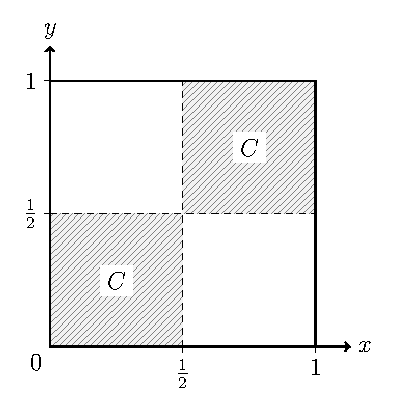
\includegraphics[width=6.5cm]{niezaleznosc-parami.pdf}
  \caption{Zdarzenie $C$ obejmuje dwa zakreskowane kwadraty.
    Zdarzeniu $A$ odpowiada prawa połowa, a $B$ górna połowa $\Omega$.}
  \label{fig:niezaleznosc-parami}
\end{figure}

\section{Własności niezależności}
\label{sec:wlasnosci-niezaleznosci}

\begin{fakt}
\label{fakt:wlasnosci-niezaleznosci}
Dla zdarzeń $A,B\in\F$ zachodzą następujące własności.
\begin{enumerate}
  \item Jeżeli $\PP(B)>0$ oraz $A,B$ są niezależne, to
    $\PP(A\mid B)=\PP(A)$.
  \item Jeżeli $A,B$ są niezależne, to niezależne są również pary
    $A,B^c$, $A^c,B$ oraz $A^c,B^c$.
  \item Jeżeli $\PP(A)=0$ lub $\PP(A)=1$, to $A$ jest niezależne
    od każdego zdarzenia $B\in\F$.
  \item Jeżeli $A$ jest niezależne od samego siebie, to
    $\PP(A)=0$ lub $\PP(A)=1$.
\end{enumerate}
\end{fakt}

\section{Schemat Bernoulliego}
\label{sec:bernoulli}

\begin{definicja}
\label{def:bernoulli}
\emph{Schematem Bernoulliego} nazywamy ciąg niezależnych powtórzeń
tego samego doświadczenia, w którym możliwe są tylko dwa wyniki:
\emph{sukces} z prawdopodobieństwem $p$ oraz \emph{porażka}
z prawdopodobieństwem $q=1-p$.
\end{definicja}

\begin{fakt}
\label{fakt:bernoulli}
W schemacie Bernoulliego prawdopodobieństwo uzyskania dokładnie $k$
sukcesów w $n$ próbach wynosi
\begin{equation}
  P_k=\binom{n}{k}p^k(1-p)^{n-k},
  \qquad k=0,1,\ldots,n.
  \label{eq:bernoulli}
\end{equation}
\end{fakt}

\begin{proof}
Przyjmujemy $\Omega=\{0,1\}^n$, gdzie $1$ oznacza sukces, a $0$ porażkę.
Dla $a=(a_1,\ldots,a_n)\in\Omega$ niezależność prób daje
\[
  \PP(\{a\})=p^{a_1+\cdots+a_n}(1-p)^{n-(a_1+\cdots+a_n)}.
\]
Zdarzenie uzyskania dokładnie $k$ sukcesów ma postać
\[
  A_k=\{(a_1,\ldots,a_n)\in\Omega:a_1+\cdots+a_n=k\}.
\]
Liczba takich ciągów wynosi $|A_k|=\binom nk$, a każdy z nich ma
prawdopodobieństwo $p^k(1-p)^{n-k}$. Zatem
\[
  \PP(A_k)=\binom nk p^k(1-p)^{n-k}.
\]
\end{proof}

\section{Granice ciągów zdarzeń}
\label{sec:granice-zdarzen}

\begin{definicja}
\label{def:granice-zdarzen}
Dla ciągu zdarzeń $(A_n)_{n\geq1}$ definiujemy \emph{granicę górną}
oraz \emph{granicę dolną} wzorami
\begin{align}
  \limsup_{n\to\infty}A_n
    &=\bigcap_{n=1}^{\infty}\bigcup_{k=n}^{\infty}A_k,
    \label{eq:limsup-zdarzen}\\
  \liminf_{n\to\infty}A_n
    &=\bigcup_{n=1}^{\infty}\bigcap_{k=n}^{\infty}A_k.
    \label{eq:liminf-zdarzen}
\end{align}
\end{definicja}

\begin{fakt}
\label{fakt:interpretacja-granic}
\leavevmode
\begin{enumerate}
  \item $\omega\in\limsup_{n\to\infty}A_n$ wtedy i tylko wtedy,
    gdy $\omega$ należy do nieskończenie wielu zdarzeń $A_n$.
  \item $\omega\in\liminf_{n\to\infty}A_n$ wtedy i tylko wtedy,
    gdy $\omega$ należy do wszystkich $A_n$ od pewnego indeksu,
    czyli do prawie wszystkich zdarzeń tego ciągu.
  \item $\displaystyle\liminf_{n\to\infty}A_n
    \subseteq\limsup_{n\to\infty}A_n$.
\end{enumerate}
\end{fakt}

\section{Lemat Borela--Cantellego}
\label{sec:borel-cantelli}

\begin{lemat}[Borela--Cantellego]
\label{lem:borel-cantelli}
Niech $(A_n)_{n\geq1}$ będzie ciągiem zdarzeń.
\begin{enumerate}
  \item Jeśli $\displaystyle\sum_{n=1}^{\infty}\PP(A_n)<\infty$, to
    \[
      \PP\!\left(\limsup_{n\to\infty}A_n\right)=0.
    \]
  \item Jeśli zdarzenia $A_n$ są niezależne i
    $\displaystyle\sum_{n=1}^{\infty}\PP(A_n)=\infty$, to
    \[
      \PP\!\left(\limsup_{n\to\infty}A_n\right)=1.
    \]
\end{enumerate}
\end{lemat}

\begin{proof}[Dowód punktu 1]
Oznaczmy $B_n=\bigcup_{k=n}^{\infty}A_k$. Ciąg $(B_n)$ jest malejący,
a jego przecięcie jest równe $\limsup_{n\to\infty}A_n$.
Z ciągłości prawdopodobieństwa dla ciągu malejącego
\eqref{eq:ciag-malejacy} oraz podaddytywności otrzymujemy
\begin{align*}
  0\leq\PP\!\left(\limsup_{n\to\infty}A_n\right)
    &=\lim_{n\to\infty}\PP(B_n)\\
    &=\lim_{n\to\infty}\PP\!\left(\bigcup_{k=n}^{\infty}A_k\right)\\
    &\leq\lim_{n\to\infty}\sum_{k=n}^{\infty}\PP(A_k)=0.
\end{align*}
Ostatnia granica jest zerowa, ponieważ są to ogony szeregu zbieżnego.
\end{proof}

\begin{proof}[Dowód punktu 2]
Ponownie korzystamy z ciągłości prawdopodobieństwa oraz z prawa de Morgana:
\begin{align*}
  \PP\!\left(\limsup_{n\to\infty}A_n\right)
    &=\lim_{n\to\infty}\PP\!\left(\bigcup_{k=n}^{\infty}A_k\right)\\
    &=1-\lim_{n\to\infty}\PP\!\left(\bigcap_{k=n}^{\infty}A_k^c\right)\\
    &=1-\lim_{n\to\infty}\lim_{N\to\infty}
      \PP\!\left(\bigcap_{k=n}^{N}A_k^c\right)\\
    &=1-\lim_{n\to\infty}\lim_{N\to\infty}
      \prod_{k=n}^{N}\bigl(1-\PP(A_k)\bigr).
\end{align*}
Ostatnia równość wynika z niezależności zdarzeń i ich dopełnień.
Z nierówności $1+x\leq e^x$, zastosowanej do $x=-\PP(A_k)$, dostajemy
\[
  0\leq\prod_{k=n}^{N}\bigl(1-\PP(A_k)\bigr)
    \leq\prod_{k=n}^{N}e^{-\PP(A_k)}
    =\exp\!\left(-\sum_{k=n}^{N}\PP(A_k)\right).
\]
Dla każdego ustalonego $n$ suma w wykładniku dąży do $+\infty$,
ponieważ $\sum_{k=1}^{\infty}\PP(A_k)=\infty$.
Stąd granica iloczynu przy $N\to\infty$ wynosi zero, a więc
\[
  1\geq\PP\!\left(\limsup_{n\to\infty}A_n\right)
    \geq1-\lim_{n\to\infty}
      \exp\!\left(-\sum_{k=n}^{\infty}\PP(A_k)\right)=1.
\]
To kończy dowód.
\end{proof}

% Źródła: materialy/2026-10-27/zmienna-losowa.png i IMG_7006--IMG_7013.jpeg.
\chapter{Zmienne losowe}
\label{chap:zmienne-losowe}

\section{Definicja i mierzalność}
\label{sec:definicja-zmiennej-losowej}

Niech $(\Omega,\F,\PP)$ będzie przestrzenią probabilistyczną.

\begin{definicja}
\label{def:zmienna-losowa}
\emph{Zmienną losową o wartościach w $\R$} na przestrzeni
$(\Omega,\F,\PP)$ nazywamy funkcję $X\colon\Omega\to\R$ taką, że
\[
  X^{-1}(A)=\{\omega\in\Omega:X(\omega)\in A\}\in\F
  \qquad\text{dla każdego }A\in\B(\R).
\]
Tutaj $\B(\R)$ oznacza $\sigma$-ciało zbiorów borelowskich prostej.
\end{definicja}

\begin{uwaga}
Analogicznie definiujemy zmienną losową $X\colon\Omega\to\R^d$,
wymagając, aby $X^{-1}(A)\in\F$ dla każdego $A\in\B(\R^d)$.
Taką zmienną nazywamy \emph{wektorem losowym}.
\end{uwaga}

\begin{uwaga}
Zmienna losowa jest funkcją mierzalną.
\end{uwaga}

\begin{uwaga}
Aby funkcja $X\colon\Omega\to\R$ była zmienną losową, wystarczy,
żeby
\[
  \{\omega\in\Omega:X(\omega)>a\}\in\F
  \qquad\text{dla każdego }a\in\R.
\]
\end{uwaga}

\begin{uwaga}[Zapis prawdopodobieństw]
Dla zbioru borelowskiego $A\subseteq\R$ stosujemy skrót
\[
  \PP(X\in A)=\PP\bigl(\{\omega\in\Omega:X(\omega)\in A\}\bigr).
\]
\end{uwaga}

\begin{uwaga}[Mierzalność funkcji]
Funkcja $f\colon(E,\mathcal E)\to(S,\mathcal S)$ jest
\emph{mierzalna}, jeżeli
\[
  f^{-1}(A)\in\mathcal E
  \qquad\text{dla każdego }A\in\mathcal S.
\]
\end{uwaga}

\begin{fakt}
\label{fakt:zlozenie-zmiennej-losowej}
Jeżeli $X\colon\Omega\to\R^d$ jest wektorem losowym, a funkcja
$\varphi\colon\R^d\to\R^m$ jest borelowska, to
\[
  \varphi(X)=\varphi\circ X\colon\Omega\to\R^m
\]
jest wektorem losowym (dla $m=1$ --- zmienną losową rzeczywistą).
\end{fakt}

\begin{uwaga}
Funkcja $\varphi\colon\R^d\to\R^m$ jest \emph{borelowska}, jeżeli
\[
  \varphi^{-1}(A)\in\B(\R^d)
  \qquad\text{dla każdego }A\in\B(\R^m).
\]
\end{uwaga}

\section{\texorpdfstring{$\sigma$}{sigma}-ciało generowane przez zmienną losową}
\label{sec:sigma-zmiennej-losowej}

\begin{definicja}
\label{def:sigma-zmiennej-losowej}
Niech $X\colon\Omega\to\R$ będzie zmienną losową.
Najmniejsze $\sigma$-ciało $\mathcal G\subseteq\F$, względem którego
$X$ jest mierzalna, nazywamy \emph{$\sigma$-ciałem generowanym przez $X$}
i oznaczamy przez $\sigma(X)$.
\end{definicja}

\begin{fakt}
\label{fakt:postac-sigma-x}
Dla zmiennej losowej $X\colon\Omega\to\R$ mamy
\[
  \sigma(X)=\{X^{-1}(B):B\in\B(\R)\}.
\]
\end{fakt}

\begin{przyklad}[Zmienna przyjmująca dwie wartości]
\label{przykl:sigma-dwie-wartosci}
Niech $A\in\F$ oraz $a,b\in\R$, $a\ne b$. Rozważmy zmienną losową
\[
  X(\omega)=a\mathbf{1}_A(\omega)+b\mathbf{1}_{A^c}(\omega),
  \qquad\omega\in\Omega,
\]
gdzie $\mathbf{1}_A$ jest funkcją wskaźnikową zbioru $A$.
Dla $B\in\B(\R)$ otrzymujemy
\[
  X^{-1}(B)=
  \begin{cases}
    \varnothing,&a\notin B,\ b\notin B,\\
    A,&a\in B,\ b\notin B,\\
    A^c,&a\notin B,\ b\in B,\\
    \Omega,&a\in B,\ b\in B.
  \end{cases}
\]
Zatem
\[
  \sigma(X)=\{\varnothing,A,A^c,\Omega\}.
\]
\end{przyklad}

\section{Niezależność zmiennych losowych}
\label{sec:niezaleznosc-zmiennych-losowych}

\begin{definicja}
\label{def:niezaleznosc-zmiennych-losowych}
Zmienne losowe $X,Y\colon\Omega\to\R$ są \emph{niezależne}, jeżeli
dla każdych $A,B\in\B(\R)$ zachodzi
\[
  \PP(X\in A,\,Y\in B)=\PP(X\in A)\PP(Y\in B).
\]
Równoważnie: $\sigma$-ciała $\sigma(X)$ i $\sigma(Y)$ są niezależne.
\end{definicja}

\begin{definicja}
\label{def:niezaleznosc-rodziny-zmiennych}
Zmienne losowe $X_1,\ldots,X_n$ są \emph{niezależne}, jeżeli
$\sigma$-ciała $\sigma(X_1)$, $\ldots$, $\sigma(X_n)$ są niezależne.
Ogólniej, dla dowolnego zbioru indeksów $T$ rodzina zmiennych losowych
$(X_t)_{t\in T}$ jest \emph{niezależna}, jeżeli rodzina
$\bigl(\sigma(X_t)\bigr)_{t\in T}$ jest niezależna.
\end{definicja}

\begin{przyklad}[Niezależne funkcje wskaźnikowe]
\label{przykl:niezalezne-wskaznikowe}
Rozważmy przestrzeń probabilistyczną
\[
  (\Omega,\F,\PP)=\bigl([0,1],\B([0,1]),\lambda\bigr),
\]
gdzie $\lambda$ oznacza miarę Lebesgue'a na odcinku $[0,1]$.
Niech
\[
  A=\left[0,\frac12\right),
  \qquad
  B=\left[0,\frac14\right)\cup\left[\frac12,\frac34\right),
  \qquad X=\mathbf{1}_A,\quad Y=\mathbf{1}_B.
\]
Wówczas
\[
  \sigma(X)=\{\varnothing,A,A^c,\Omega\},
  \qquad
  \sigma(Y)=\{\varnothing,B,B^c,\Omega\}.
\]
Ponadto
\[
  \PP(A\cap B)
    =\lambda\!\left(\left[0,\frac14\right)\right)
    =\frac14=\frac12\cdot\frac12=\PP(A)\PP(B).
\]
Zdarzenia $A,B$ są niezależne, a z własności niezależności
(fakt~\ref{fakt:wlasnosci-niezaleznosci}) to samo dotyczy ich dopełnień.
Zatem $\sigma$-ciała $\sigma(X)$ i $\sigma(Y)$ są niezależne,
czyli zmienne losowe $X,Y$ są niezależne.
\end{przyklad}

\begin{przyklad}[Funkcje Rademachera]
\label{przykl:rademacher}
Na tej samej przestrzeni probabilistycznej funkcje
\[
  X_n(x)=\operatorname{sgn}\!\bigl(\sin(2^n\pi x)\bigr),
  \qquad x\in[0,1],\quad n=1,2,\ldots,
\]
tworzą rodzinę niezależnych zmiennych losowych.
Zera sinusów występują w punktach dyadycznych, w tym na końcach odcinka;
zbiór tych punktów ma miarę zero, więc wartości funkcji w tych punktach
nie wpływają na niezależność.
\end{przyklad}

\begin{fakt}
\label{fakt:zmienna-niezalezna-od-siebie}
Zmienna losowa $X\colon\Omega\to\R$ jest niezależna od samej siebie
wtedy i tylko wtedy, gdy istnieje $c\in\R$ takie, że
\[
  \PP(X=c)=1.
\]
\end{fakt}

\section{Układy \texorpdfstring{$\pi$ i $\lambda$}{pi i lambda}}
\label{sec:pi-lambda}

\begin{definicja}
\label{def:pi-uklad}
Rodzinę zbiorów $\mathcal P\subseteq2^\Omega$ nazywamy
\emph{$\pi$-układem}, jeżeli
\[
  A\cap B\in\mathcal P
  \qquad\text{dla wszystkich }A,B\in\mathcal P.
\]
\end{definicja}

\begin{przyklad}
Rodzina
\[
  \mathcal P=\{[a,b):a,b\in\R\}
\]
jest $\pi$-układem na $\R$. Przyjmujemy przy tym $[a,b)=\varnothing$
dla $a\geq b$.
\end{przyklad}

\begin{definicja}
\label{def:lambda-uklad}
Rodzinę zbiorów $\mathcal L\subseteq2^\Omega$ nazywamy
\emph{$\lambda$-układem}, jeżeli spełnia następujące warunki:
\begin{enumerate}
  \item $\Omega\in\mathcal L$.
  \item Jeżeli $A,B\in\mathcal L$ i $A\subseteq B$, to
    $B\setminus A\in\mathcal L$.
  \item Jeżeli $A_1,A_2,\ldots\in\mathcal L$ oraz
    $A_n\subseteq A_{n+1}$ dla każdego $n\geq1$, to
    \[
      \bigcup_{n=1}^{\infty}A_n\in\mathcal L.
    \]
\end{enumerate}
\end{definicja}

\begin{fakt}
\label{fakt:pi-lambda-sigma}
Jeżeli rodzina $\F$ jest jednocześnie $\pi$-układem i $\lambda$-układem,
to jest $\sigma$-ciałem.
\end{fakt}

\begin{twierdzenie}[O układach $\pi$ i $\lambda$]
\label{tw:pi-lambda}
Jeżeli $\lambda$-układ $\mathcal L$ zawiera $\pi$-układ $\mathcal P$,
to
\[
  \sigma(\mathcal P)\subseteq\mathcal L.
\]
\end{twierdzenie}

\subsection{Sposób stosowania twierdzenia}
\label{subsec:stosowanie-pi-lambda}

Chcąc udowodnić pewną własność $(\ast)$ dla każdego $A\in\F$,
możemy postępować następująco:
\begin{enumerate}
  \item Znajdujemy $\pi$-układ $\mathcal P$ taki, że
    $\sigma(\mathcal P)=\F$, i sprawdzamy własność $(\ast)$
    dla każdego zbioru z $\mathcal P$.
  \item Definiujemy rodzinę
    \[
      \mathcal L=\{A\in\F:\text{własność }(\ast)\text{ zachodzi dla }A\}.
    \]
  \item Wykazujemy, że $\mathcal L$ jest $\lambda$-układem.
  \item Ponieważ $\mathcal P\subseteq\mathcal L$, z
    twierdzenia~\ref{tw:pi-lambda} otrzymujemy
    \[
      \F=\sigma(\mathcal P)\subseteq\mathcal L.
    \]
    Własność $(\ast)$ zachodzi więc dla każdego $A\in\F$.
\end{enumerate}

% Źródła: materialy/2026-10-29/IMG_7038--IMG_7043.jpeg.
\poczatekwykladu{5}

\section{Funkcje niezależnych zmiennych losowych}
\label{sec:funkcje-niezaleznych-zmiennych}

\begin{twierdzenie}
\label{tw:funkcje-niezaleznych-blokow}
Niech $X_1,\ldots,X_{n+m}$ będą niezależnymi zmiennymi losowymi,
gdzie $n,m\geq1$. Wówczas dla dowolnych zbiorów borelowskich
$C\in\B(\R^n)$ i $D\in\B(\R^m)$ zdarzenia
\[
  \{(X_1,\ldots,X_n)\in C\},
  \qquad
  \{(X_{n+1},\ldots,X_{n+m})\in D\}
\]
są niezależne. W szczególności, jeżeli funkcje
\[
  f\colon\R^n\to\R,
  \qquad g\colon\R^m\to\R
\]
są borelowskie, to zmienne losowe
\[
  f(X_1,\ldots,X_n),
  \qquad g(X_{n+1},\ldots,X_{n+m})
\]
są niezależne.
\end{twierdzenie}

\begin{uwaga}[Więcej bloków]
\label{uwaga:wiecej-niezaleznych-blokow}
Ogólniej, niech $X_1,\ldots,X_n$ będą niezależne oraz
\[
  0=n_0<n_1<\cdots<n_k=n.
\]
Jeżeli dla $i=1,\ldots,k$ funkcje
$f_i\colon\R^{n_i-n_{i-1}}\to\R$ są borelowskie, to zmienne
\[
  f_1(X_1,\ldots,X_{n_1}),\quad
  f_2(X_{n_1+1},\ldots,X_{n_2}),\quad\ldots,\quad
  f_k(X_{n_{k-1}+1},\ldots,X_n)
\]
są niezależne.
\end{uwaga}

\begin{przyklad}
Jeżeli $X_1,X_2,X_3$ są niezależne, to
$\sin(X_1+X_2)$ i $e^{X_3}$ są niezależne.
Podobnie z niezależności $X_1,X_2,X_3,X_4$ wynika niezależność
zmiennych $X_1+X_2$ oraz $X_3-X_4$.
\end{przyklad}

\begin{uwaga}
Twierdzenie dotyczy funkcji oddzielnych bloków zmiennych.
Z samej niezależności $X_1$ i $X_2$ nie można wnioskować,
że zmienne $X_1+X_2$ oraz $X_1-X_2$ są niezależne.
\end{uwaga}

\begin{proof}[Szkic dowodu twierdzenia~\ref{tw:funkcje-niezaleznych-blokow}]
Oznaczmy
\[
  X=(X_1,\ldots,X_n),
  \qquad Y=(X_{n+1},\ldots,X_{n+m}).
\]
Chcemy wykazać, że
\begin{equation}
  \PP(X\in C,\,Y\in D)=\PP(X\in C)\PP(Y\in D)
  \label{eq:niezaleznosc-blokow}
\end{equation}
dla wszystkich $C\in\B(\R^n)$ oraz $D\in\B(\R^m)$.

Dla $d\geq1$ rozważmy rodzinę prostokątów
\[
  \mathcal A^d=
  \left\{\prod_{i=1}^d[a_i,b_i):
    a_i,b_i\in\R,\ a_i\leq b_i\right\}.
\]
Jest to $\pi$-układ i $\sigma(\mathcal A^d)=\B(\R^d)$.
Przypadek $d=2$ przedstawia rysunek~\ref{fig:prostokat-borelowski}.

\begin{figure}[H]
  \centering
  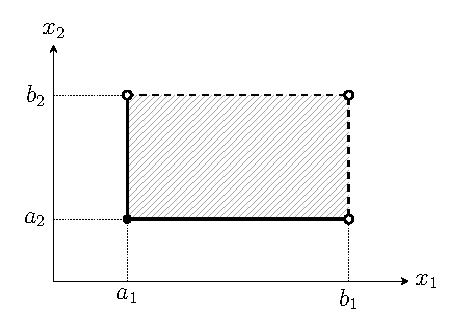
\includegraphics[width=5.4cm]{prostokat-borelowski.pdf}
  \caption{Prostokąt $[a_1,b_1)\times[a_2,b_2)$.
    Dolne końce obu przedziałów są włączone, górne wyłączone.}
  \label{fig:prostokat-borelowski}
\end{figure}

\emph{Krok 1.} Ustalmy $D\in\mathcal A^m$ i zdefiniujmy
\[
  \mathcal L_1=
  \{C\in\B(\R^n):\text{równość~\eqref{eq:niezaleznosc-blokow}
    zachodzi dla }C,D\}.
\]
Rodzina $\mathcal L_1$ jest $\lambda$-układem: zawiera $\R^n$,
jest zamknięta na różnice zbiorów zagnieżdżonych oraz na sumy
ciągów rosnących. Wynika to odpowiednio z normalizacji,
addytywności i ciągłości prawdopodobieństwa.

Jeżeli również $C\in\mathcal A^n$, to możemy zapisać
\[
  C=\prod_{i=1}^n[a_i,b_i),
  \qquad
  D=\prod_{i=n+1}^{n+m}[a_i,b_i).
\]
Z niezależności wszystkich zmiennych otrzymujemy
\begin{align*}
  \PP(X\in C,\,Y\in D)
    &=\PP\!\left(\bigcap_{i=1}^{n+m}\{X_i\in[a_i,b_i)\}\right)\\
    &=\prod_{i=1}^{n+m}\PP(X_i\in[a_i,b_i))\\
    &=\left(\prod_{i=1}^{n}\PP(X_i\in[a_i,b_i))\right)
      \left(\prod_{i=n+1}^{n+m}\PP(X_i\in[a_i,b_i))\right)\\
    &=\PP(X\in C)\PP(Y\in D).
\end{align*}
Zatem $\mathcal A^n\subseteq\mathcal L_1$. Na mocy twierdzenia
o układach $\pi$ i $\lambda$ (twierdzenie~\ref{tw:pi-lambda})
\[
  \B(\R^n)=\sigma(\mathcal A^n)\subseteq\mathcal L_1.
\]
Równość~\eqref{eq:niezaleznosc-blokow} zachodzi więc dla każdego
$C\in\B(\R^n)$ i ustalonego $D\in\mathcal A^m$.

\emph{Krok 2.} Ustalmy teraz dowolny $C\in\B(\R^n)$ i połóżmy
\[
  \mathcal L_2=
  \{D\in\B(\R^m):\text{równość~\eqref{eq:niezaleznosc-blokow}
    zachodzi dla }C,D\}.
\]
Rodzina $\mathcal L_2$ również jest $\lambda$-układem.
Z poprzedniego kroku wynika $\mathcal A^m\subseteq\mathcal L_2$.
Ponownie stosując twierdzenie~\ref{tw:pi-lambda}, dostajemy
\[
  \B(\R^m)=\sigma(\mathcal A^m)\subseteq\mathcal L_2.
\]
Dowodzi to niezależności wektorów $X$ i $Y$.

\emph{Krok 3.} Niech $f\colon\R^n\to\R$ i $g\colon\R^m\to\R$
będą borelowskie. Dla dowolnych $E,F\in\B(\R)$ przeciwobrazy
$f^{-1}(E)\in\B(\R^n)$ i $g^{-1}(F)\in\B(\R^m)$ są borelowskie.
Wobec tego
\begin{align*}
  \PP(f(X)\in E,\,g(Y)\in F)
    &=\PP\bigl(X\in f^{-1}(E),\,Y\in g^{-1}(F)\bigr)\\
    &=\PP\bigl(X\in f^{-1}(E)\bigr)
      \PP\bigl(Y\in g^{-1}(F)\bigr)\\
    &=\PP(f(X)\in E)\PP(g(Y)\in F).
\end{align*}
Zatem $f(X)$ i $g(Y)$ są niezależne.
\end{proof}

% Źródła: materialy/2026-10-29/IMG_7044--IMG_7050.jpeg.
\chapter{Rozkłady zmiennych losowych}
\label{chap:rozklady-zmiennych-losowych}

\section{Rozkład prawdopodobieństwa}
\label{sec:rozklad-prawdopodobienstwa}

\begin{definicja}
\label{def:rozklad-prawdopodobienstwa}
\emph{Rozkładem prawdopodobieństwa na $\R^n$} nazywamy każdą miarę
probabilistyczną $\mu$ na przestrzeni mierzalnej $(\R^n,\B(\R^n))$,
czyli miarę taką, że $\mu(\R^n)=1$.
\end{definicja}

\begin{definicja}
\label{def:rozklad-zmiennej-losowej}
Niech $X\colon\Omega\to\R^n$ będzie wektorem losowym na przestrzeni
$(\Omega,\F,\PP)$. \emph{Rozkład zmiennej losowej $X$} to miara
$\mu_X$ określona wzorem
\[
  \mu_X(A)=\PP(X\in A)=\PP\bigl(X^{-1}(A)\bigr),
  \qquad A\in\B(\R^n).
\]
\end{definicja}

W szczególności
\[
  \mu_X(\R^n)=\PP(X\in\R^n)=\PP(\Omega)=1.
\]
Schemat przejścia od zdarzenia w przestrzeni wyników do zbioru wartości
zmiennej przedstawia rysunek~\ref{fig:schemat-rozkladu}.

\begin{figure}[H]
  \centering
  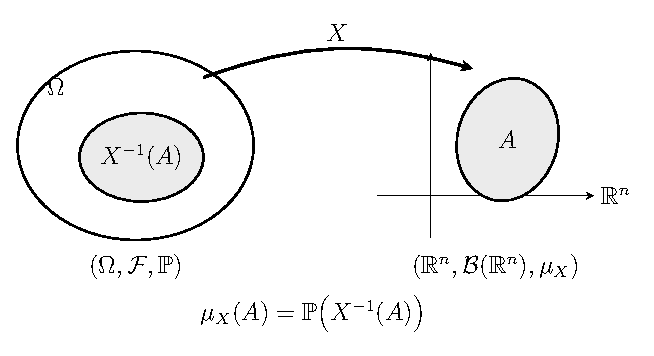
\includegraphics[width=10.5cm]{schemat-rozkladu.pdf}
  \caption{Zbiorowi borelowskiemu $A\subseteq\R^n$ odpowiada zdarzenie
    $X^{-1}(A)\subseteq\Omega$.
    Rozkład przypisuje mu masę $\mu_X(A)=\PP(X^{-1}(A))$.}
  \label{fig:schemat-rozkladu}
\end{figure}

\begin{przyklad}[Trzy zmienne na odcinku jednostkowym]
\label{przykl:trzy-rozklady}
Rozważmy przestrzeń probabilistyczną
\[
  (\Omega,\F,\PP)=\bigl([0,1],\B([0,1]),\lambda\bigr),
\]
gdzie $\lambda$ jest miarą Lebesgue'a na $[0,1]$.

\emph{a) Zmienna stała.} Niech $X(\omega)=c$ dla każdego $\omega\in[0,1]$,
gdzie $c\in\R$. Dla $A\in\B(\R)$ mamy
\[
  \mu_X(A)=\PP(X\in A)=
  \begin{cases}
    1,&c\in A,\\
    0,&c\notin A.
  \end{cases}
\]
Jest to \emph{miara Diraca w punkcie $c$}, oznaczana przez $\delta_c$.

\emph{b) Indykator.} Niech
\[
  Y(\omega)=\mathbf{1}_{[0,\,2/3)}(\omega).
\]
Wówczas dla każdego $A\in\B(\R)$
\[
  \mu_Y(A)=
  \begin{cases}
    1,&0\in A,\ 1\in A,\\[2pt]
    \dfrac13,&0\in A,\ 1\notin A,\\[5pt]
    \dfrac23,&0\notin A,\ 1\in A,\\[5pt]
    0,&0\notin A,\ 1\notin A.
  \end{cases}
\]
Możemy zatem zapisać
\[
  \mu_Y=\frac13\delta_0+\frac23\delta_1.
\]

\emph{c) Zmienna identycznościowa.} Dla $Z(\omega)=\omega$, $\omega\in[0,1]$,
otrzymujemy
\[
  \mu_Z(A)=\PP(Z\in A)=\lambda\bigl([0,1]\cap A\bigr),
  \qquad A\in\B(\R).
\]
Wykresy zmiennych z tego przykładu pokazano na
rysunku~\ref{fig:trzy-zmienne}.
\end{przyklad}

\begin{figure}[H]
  \centering
  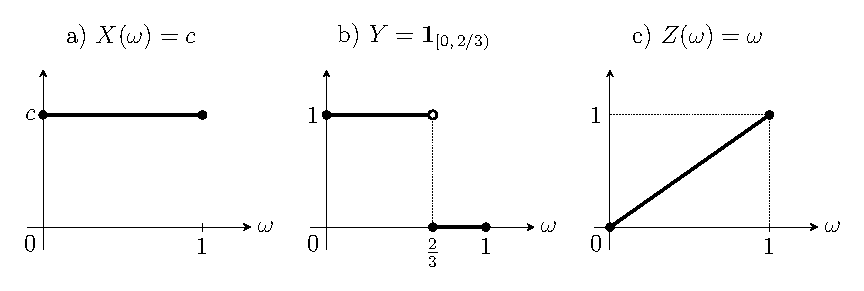
\includegraphics[width=\textwidth]{przyklady-zmiennych.pdf}
  \caption{Wykresy trzech zmiennych z przykładu~\ref{przykl:trzy-rozklady}.
    Są to wykresy funkcji na $\Omega=[0,1]$.}
  \label{fig:trzy-zmienne}
\end{figure}

\begin{przyklad}[Liczba szóstek]
\label{przykl:rozklad-liczby-szostek}
Rzucamy niezależnie $n$ razy uczciwą kostką. Niech $X$ oznacza liczbę
szóstek w tych rzutach. Wówczas
\[
  \mu_X(\{k\})=\PP(X=k)
    =\binom nk\left(\frac16\right)^k\left(\frac56\right)^{n-k},
  \qquad k=0,1,\ldots,n.
\]
Zmienna $X$ nie przyjmuje innych wartości, więc na przykład
\[
  \mu_X\!\left(\left\{\frac32\right\}\right)=0,
  \qquad \mu_X(\{n+1\})=0.
\]
Dla dowolnego $A\in\B(\R)$ mamy
\begin{align*}
  \mu_X(A)
    &=\sum_{k=0}^n\PP(X=k)\delta_k(A)\\
    &=\sum_{k=0}^n\binom nk
      \left(\frac16\right)^k\left(\frac56\right)^{n-k}\delta_k(A).
\end{align*}
\end{przyklad}

\section{Rozkłady dyskretne}
\label{sec:rozklady-dyskretne}

\begin{definicja}
\label{def:rozklad-dyskretny}
Niech $X\colon\Omega\to\R$ będzie zmienną losową. Definiujemy
\[
  S_X=\{x\in\R:\mu_X(\{x\})=\PP(X=x)>0\}.
\]
Mówimy, że $X$ ma \emph{rozkład dyskretny}, jeżeli
\[
  \PP(X\in S_X)=1.
\]
\end{definicja}

\begin{uwaga}
Mówimy, że rozkład zmiennej $X$ jest \emph{skupiony na zbiorze $A$},
jeżeli $A\in\B(\R)$ oraz $\PP(X\in A)=1$.
\end{uwaga}

\begin{fakt}
\label{fakt:przeliczalnosc-atomow}
Zbiór $S_X$ jest co najwyżej przeliczalny.
\end{fakt}
\noindent\emph{Dowód pozostawiono jako ćwiczenie.}

\begin{fakt}
\label{fakt:opis-rozkladu-dyskretnego}
Rozkład dyskretny jest jednoznacznie wyznaczony przez zbiór
\[
  S_X=\{x_n:n\in T\},
\]
gdzie $T$ jest co najwyżej przeliczalnym zbiorem indeksów, punkty $x_n$
są różne, oraz przez liczby
\[
  p_n=\PP(X=x_n),\qquad n\in T.
\]
Wówczas
\[
  \sum_{n\in T}p_n=1,
  \qquad
  \mu_X(A)=\PP(X\in A)=\sum_{\substack{n\in T\\x_n\in A}}p_n,
  \quad A\in\B(\R).
\]
\end{fakt}

\subsection{Przykłady rozkładów dyskretnych}
\label{subsec:przyklady-rozkladow-dyskretnych}

\begin{przyklad}[Rozkład skupiony w jednym punkcie]
Dla $a\in\R$ rozkład $\mu=\delta_a$ spełnia
\[
  \mu(A)=\delta_a(A),\qquad A\in\B(\R).
\]
Zmienna o tym rozkładzie spełnia $\PP(X=a)=1$.
\end{przyklad}

\begin{przyklad}[Rozkład dwupunktowy]
Niech $p\in[0,1]$ oraz $q=1-p$. Jeżeli
\[
  \PP(X=1)=p,\qquad\PP(X=0)=q,
\]
to
\[
  \mu_X=p\delta_1+(1-p)\delta_0.
\]
Ogólniej, rozkład skupiony na dwóch różnych punktach $x_1,x_2$ ma postać
$\alpha\delta_{x_1}+(1-\alpha)\delta_{x_2}$ dla pewnego $\alpha\in[0,1]$.
\end{przyklad}

\begin{przyklad}[Rozkład Bernoulliego]
\label{przykl:rozklad-bernoulliego}
Rozkład Bernoulliego $B(n,p)$, gdzie $n\geq1$ i $p\in[0,1]$,
jest określony przez
\[
  \PP(X=k)=\binom nk p^k(1-p)^{n-k},
  \qquad k=0,1,\ldots,n.
\]
W przypadkach brzegowych stosujemy konwencję $0^0=1$.
\end{przyklad}

\begin{przyklad}[Rozkład geometryczny]
\label{przykl:rozklad-geometryczny}
Dla $p\in(0,1]$ rozkład geometryczny, oznaczany przez $G(p)$,
jest dany wzorem
\[
  \PP(X=k)=(1-p)^{k-1}p,\qquad k=1,2,\ldots.
\]
Piszemy wówczas $X\sim G(p)$; dla $p=1$ cała masa jest skupiona w punkcie $1$.
\end{przyklad}

\begin{przyklad}[Rozkład Poissona]
\label{przykl:rozklad-poissona}
Rozkład Poissona o parametrze $\lambda\geq0$, oznaczany przez
$\operatorname{Pois}(\lambda)$, jest określony przez
\[
  \PP(X=k)=\frac{\lambda^k}{k!}e^{-\lambda},
  \qquad k=0,1,2,\ldots.
\]
Piszemy $X\sim\operatorname{Pois}(\lambda)$.
Dla $\lambda=0$ rozkład jest równy $\delta_0$.
\end{przyklad}


\end{document}
